% !TEX root = ../main.tex
\section{Appendix}

\begin{figure}[H]
\centering
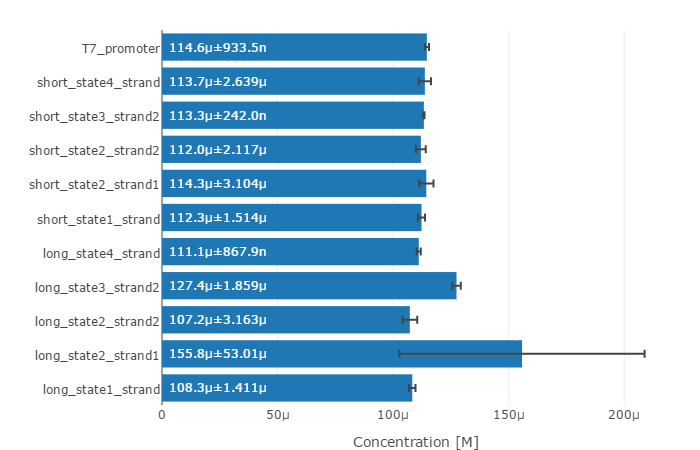
\includegraphics[width=\columnwidth]{images/oligo_concentrations.png}
\caption{Concentrations of the dissolved DNA oligos ordered from IDT.}
\label{oligo_concentrations}
\end{figure}

\begin{figure}[H]
\centering
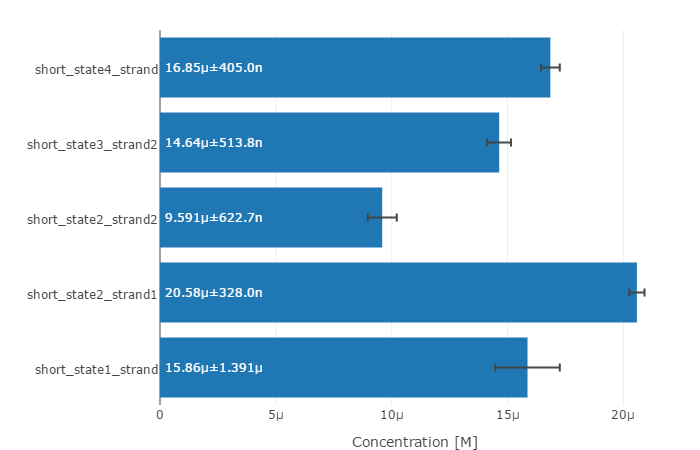
\includegraphics[width=\columnwidth]{images/translator_transcription_concentration.png}
\caption{Concentrations of the short translator RNA sequences.}
\label{translator_transcription_concentration}
\end{figure}


\begin{figure}
\begin{subfigure}{.32\columnwidth}
  \centering
  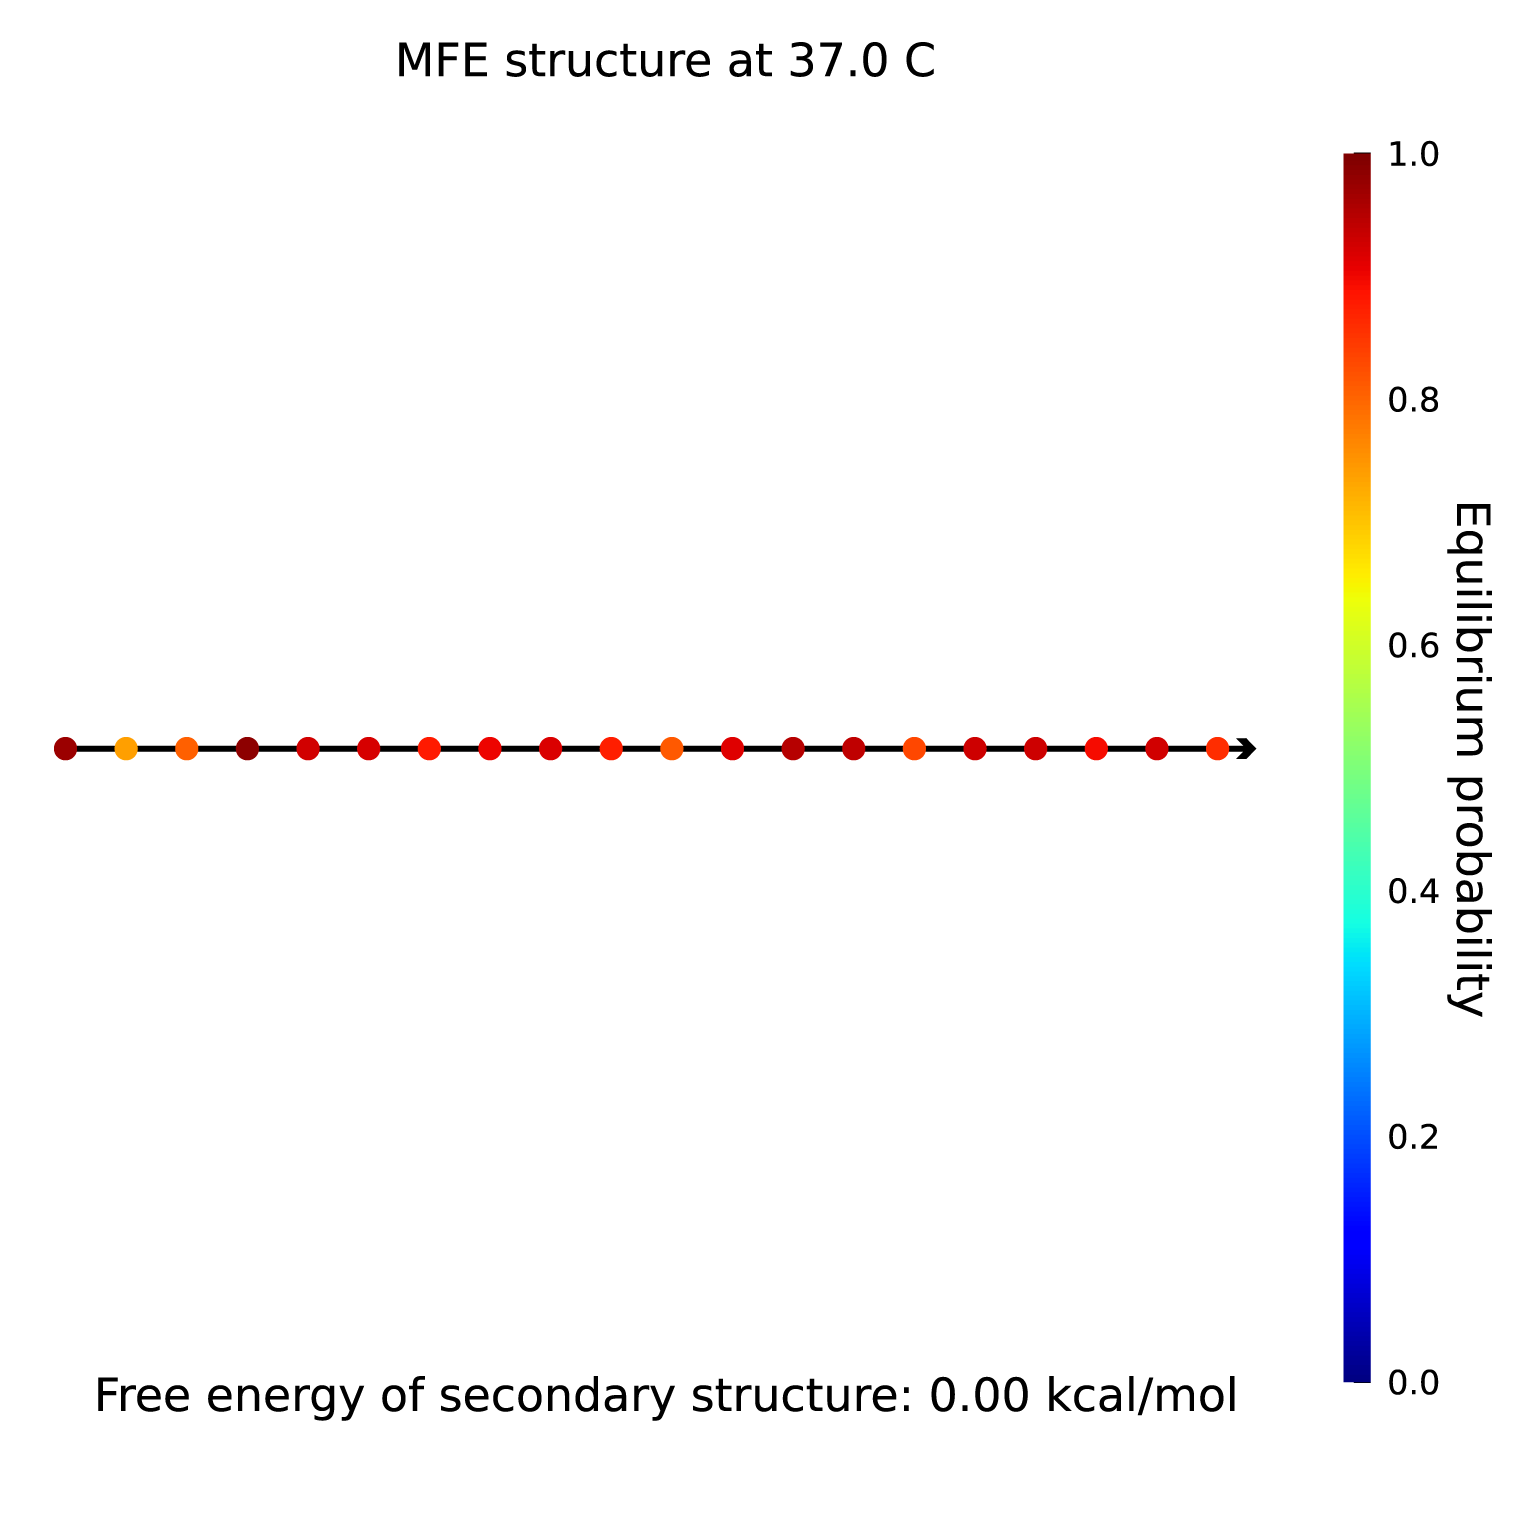
\includegraphics[width=\linewidth]{images/0_analysis.png}
  \caption{T7 promoter}
\end{subfigure}%
\begin{subfigure}{.32\columnwidth}
  \centering
  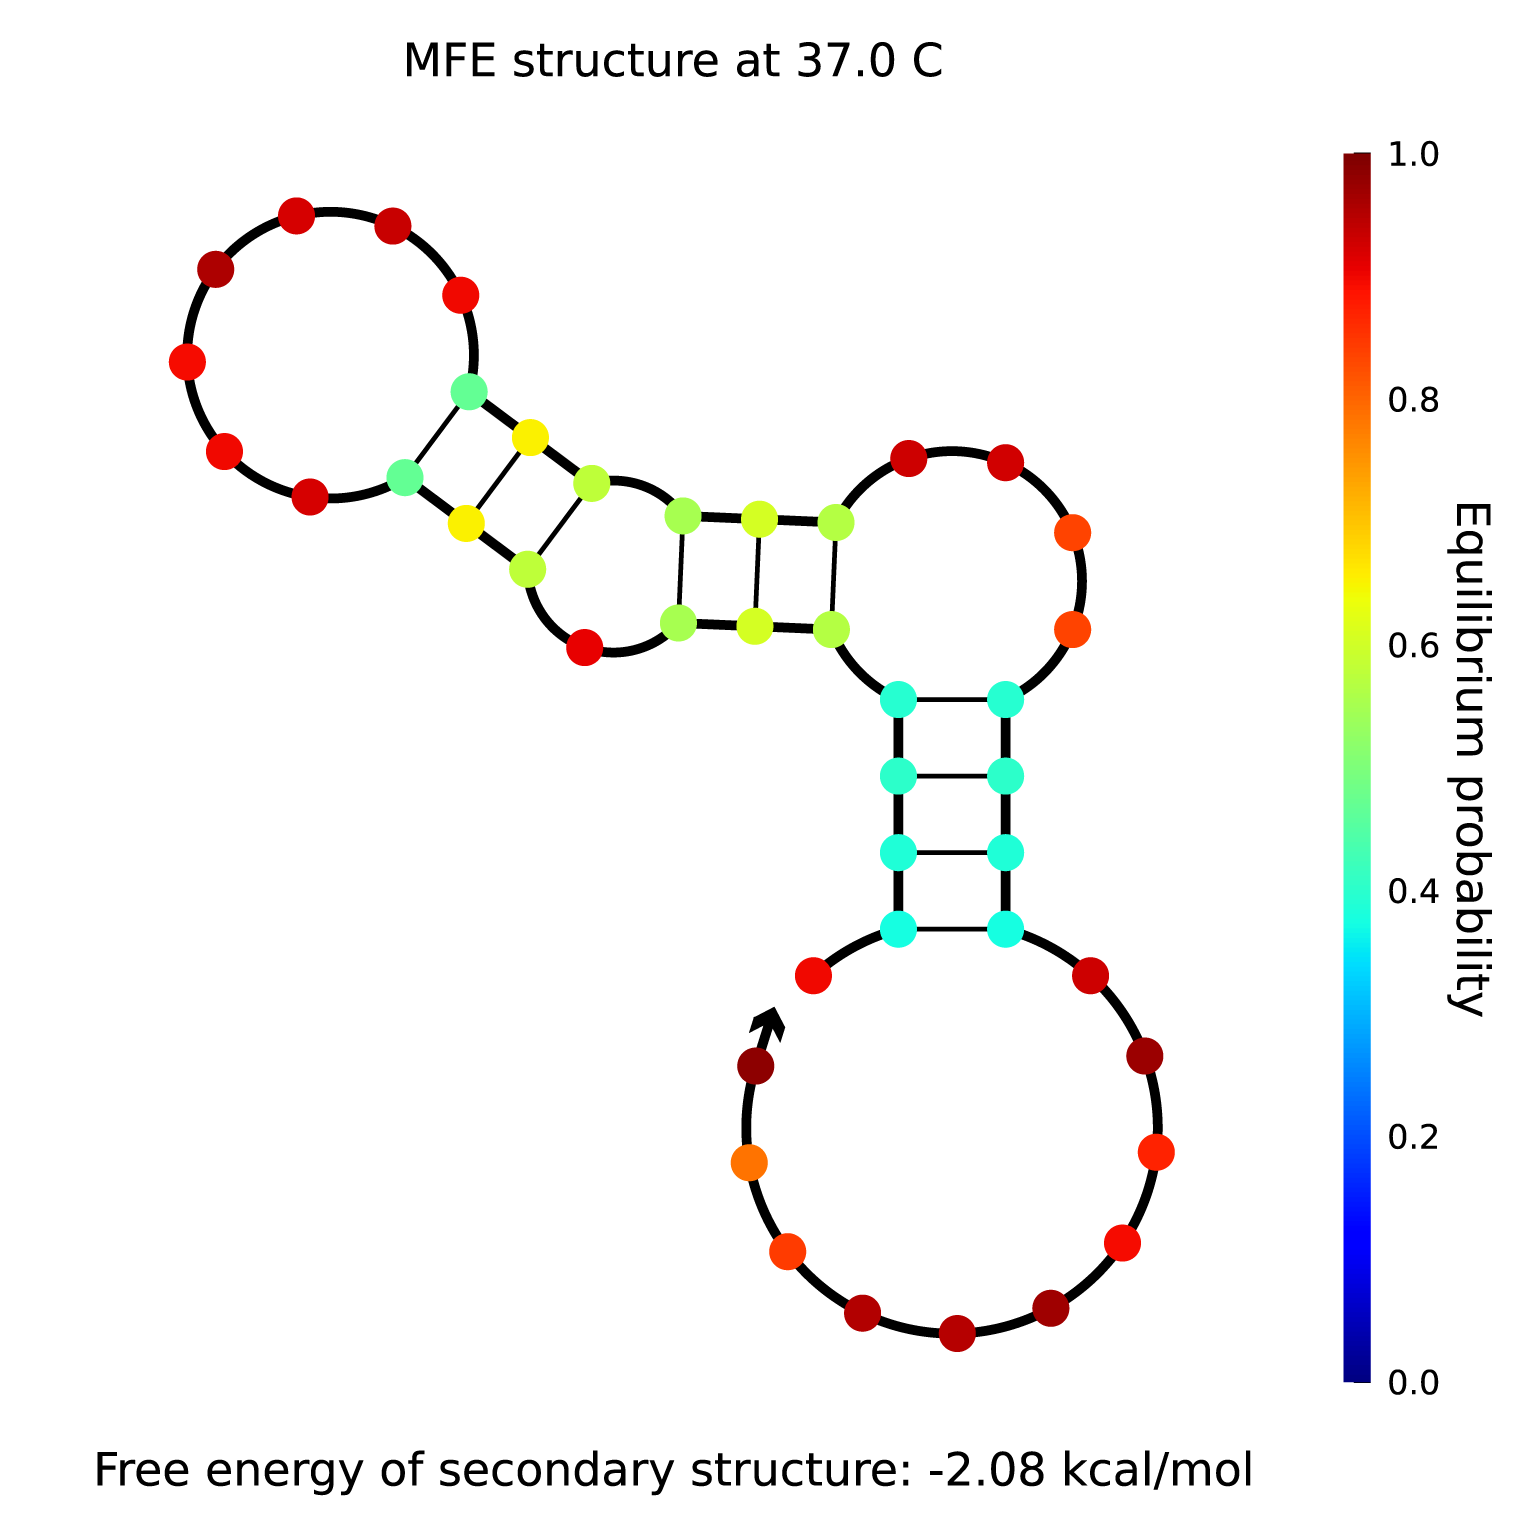
\includegraphics[width=\linewidth]{images/1_analysis.png}
  \caption{Short 1}
\end{subfigure}
\begin{subfigure}{.32\columnwidth}
  \centering
  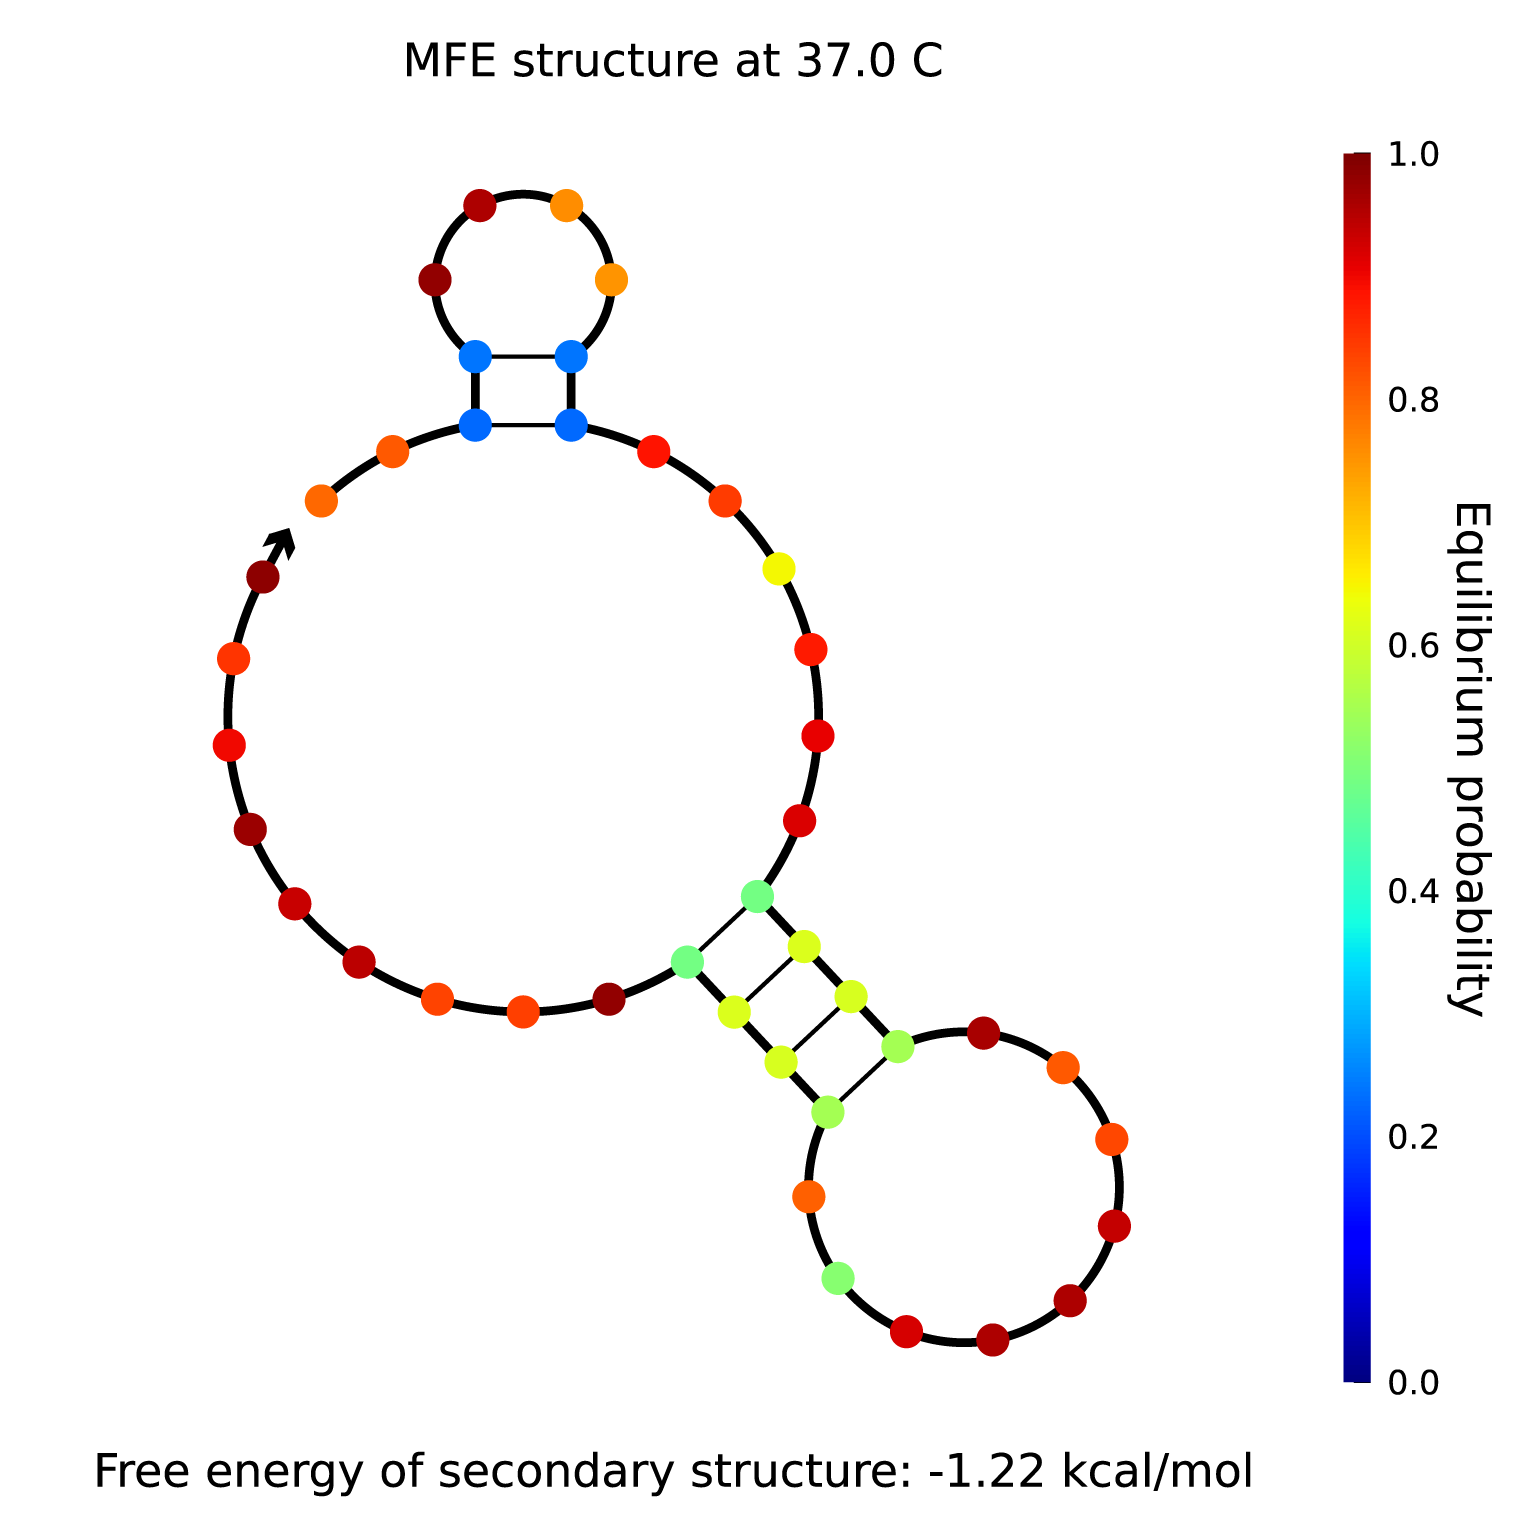
\includegraphics[width=\linewidth]{images/2_analysis.png}
  \caption{Short 2}
\end{subfigure}
\begin{subfigure}{.32\columnwidth}
  \centering
  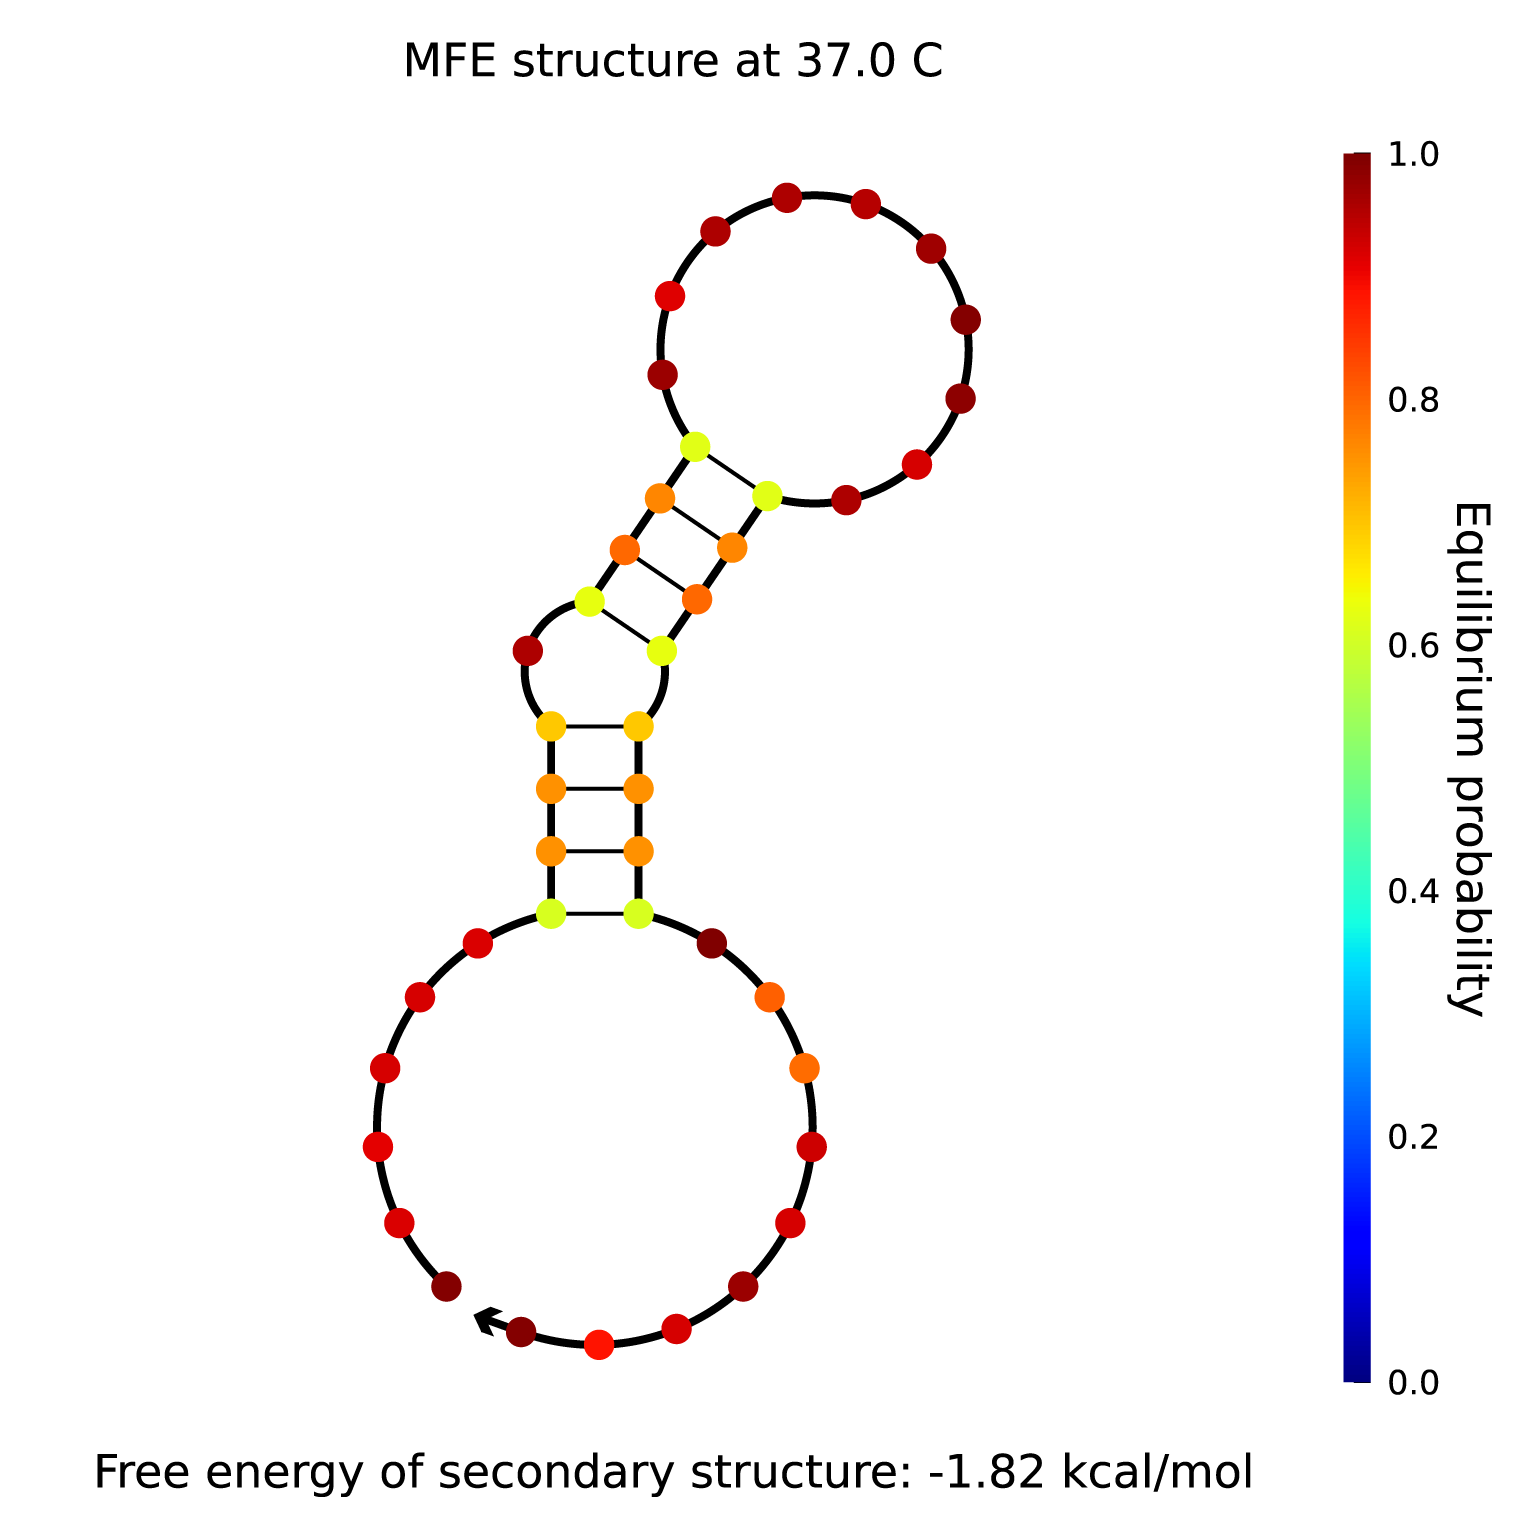
\includegraphics[width=\linewidth]{images/3_analysis.png}
  \caption{Short 3}
\end{subfigure}
\begin{subfigure}{.32\columnwidth}
  \centering
  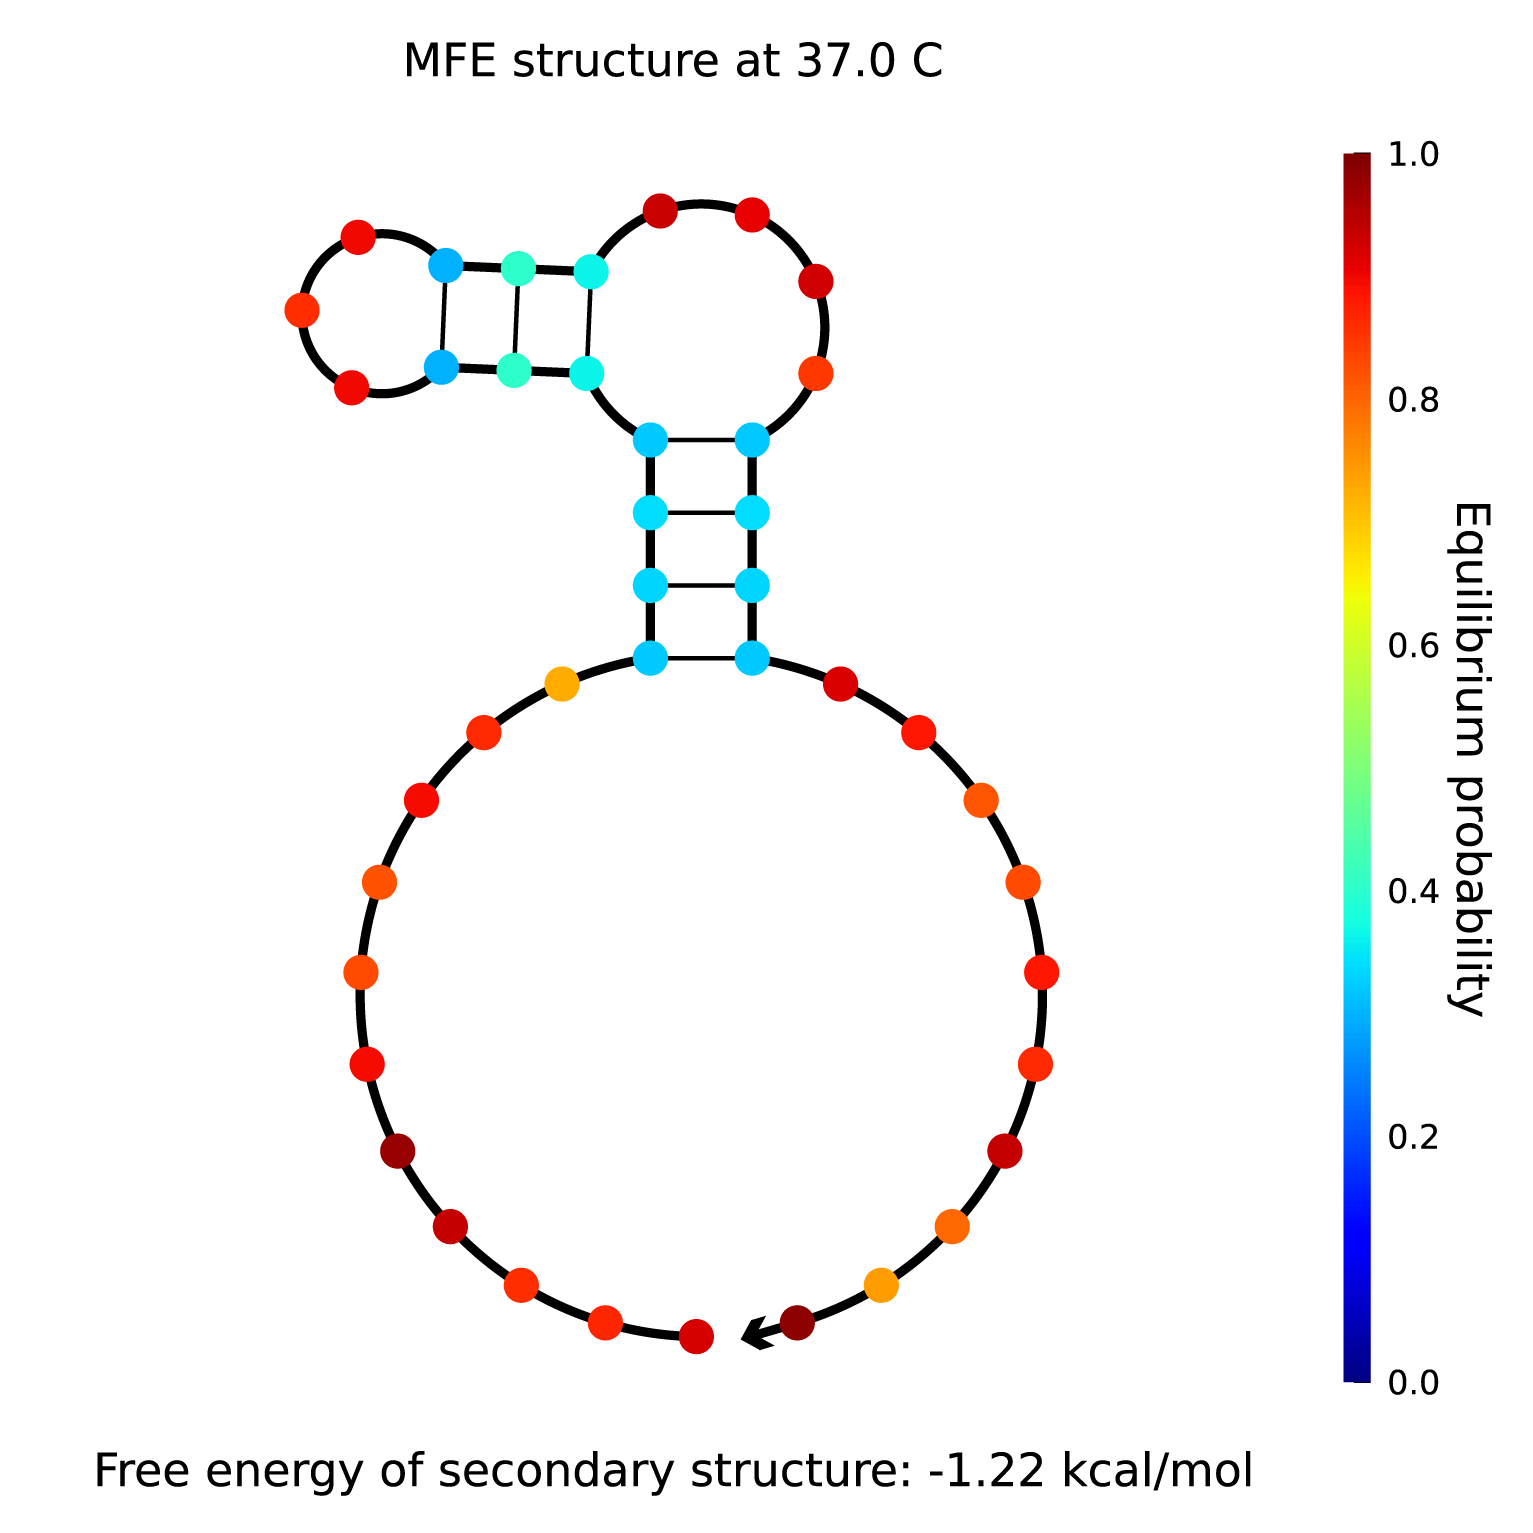
\includegraphics[width=\linewidth]{images/4_analysis.png}
  \caption{Short 4}
\end{subfigure}
\begin{subfigure}{.32\columnwidth}
  \centering
  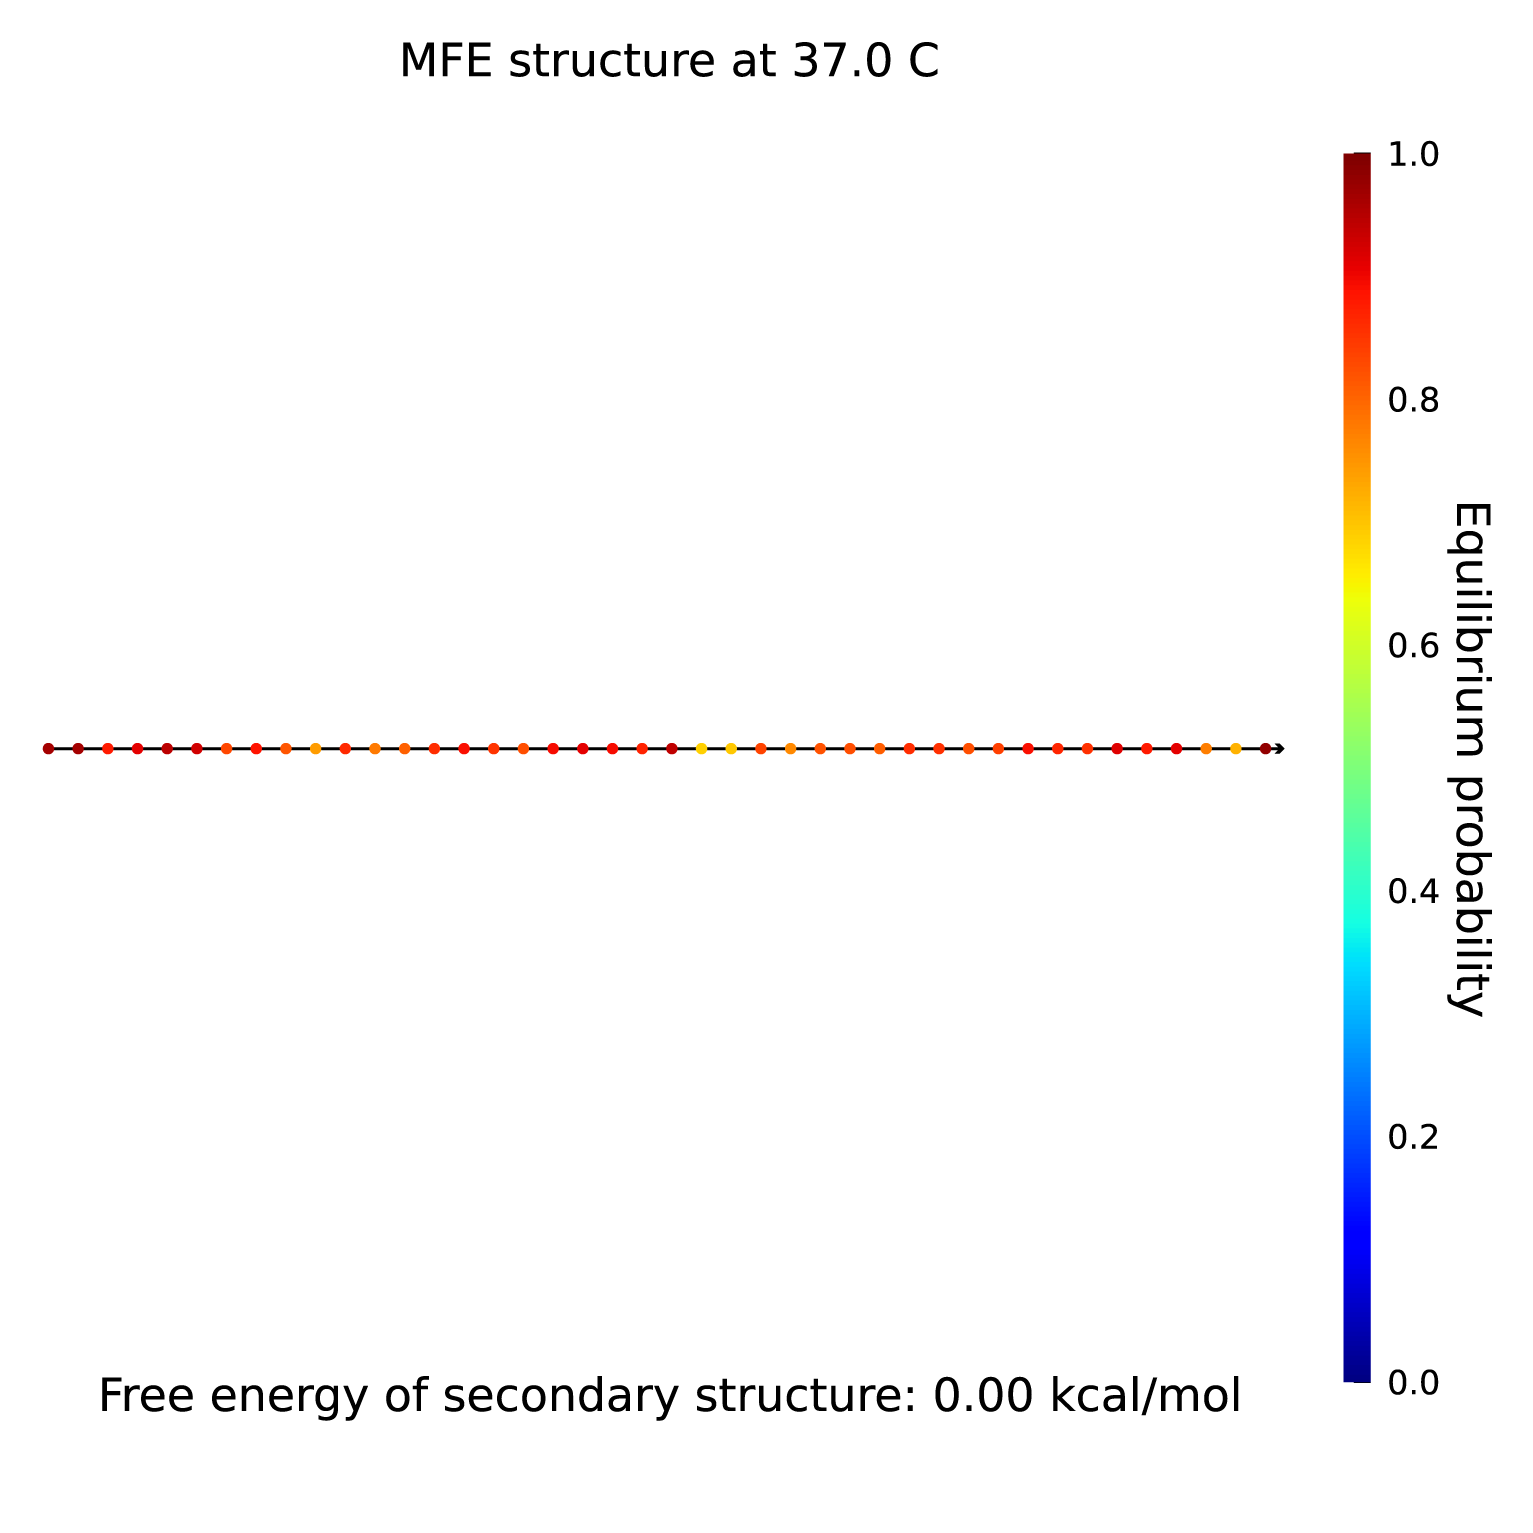
\includegraphics[width=\linewidth]{images/5_analysis.png}
  \caption{Short 5}
\end{subfigure}
\caption{Secondary structures of the DNA sequences for the short translator and the T7 promoter sequence.}
\label{short_secondary_structures}
\end{figure}
